\documentclass[10pt]{scrartcl}
\usepackage[utf8]{inputenc}
\usepackage{graphicx} 
\author{Dane Wicki}
\title{Universal data acquisition}
\subtitle{FS17 Praxismodul}
\renewcommand{\contentsname}{Inhaltsverzeichnis}
\begin{document}
\maketitle
\tableofcontents
\newpage

\section{Einleitung, Problembeschreibung}
\subsection{Gescheftsfeld der Firma}
Die Siemens AG ist ein führender internationaler Technologiekonzern, der seit mehr als 165 Jahren für technische Leistungsfähigkeit, Innovation, Qualität, Zuverlässigkeit und Internationalität steht. Das Unternehmen ist in mehr als 200 Ländern aktiv, und zwar schwerpunktmäßig auf den Gebieten Elektrifizierung, Automatisierung und Digitalisierung. Siemens ist weltweit einer der größten Hersteller energieeffizienter ressourcenschonender Technologien. Das Unternehmen ist einer der führenden Anbieter effizienter Energieerzeugungs- und Energieübertragungslösungen, Pionier bei Infrastrukturlösungen sowie bei Automatisierungs-, Antriebs- und Softwarelösungen für die Industrie. Darüber hinaus ist das Unternehmen ein führender Anbieter bildgebender medizinischer Geräte wie Computertomographen und Magnetresonanztomographen sowie in der Labordiagnostik und klinischer IT.
\subsection{Projektkontext}
Die Firma Siemens BT in Zug ist zuständig für die Entwicklung von Brandmeldern.
Um die Qualität der Brandmelder zu gewährleisten, werden diese unter Zuhilfenahme
verschiedener Apparaturen und Testaufbauten getestet. Dies geschieht bei vielen Aufbauten automatisch und mit konsistenter Aufzeichnung der Daten, welche der Melder und etwaige Referenz-Geräte erzeugen. Es gibt jedoch weiterhin aufbauten, bei welchen die Aufzeichnung weder Automatisch noch Konsistent gespeichert werden kann oder nur unter grossen Anstrengungen der Arbeitenden. Diesen Zustand gilt es nun zu verbessern.
Dazu soll eine Software entwickelt werden, die aus verschiedenen Ressourcen (verschiedenen
Datenquellen) die Daten sammelt und diese in eine auswertbare Excel-Datei exportiert. Dies
Software basiert auf einer bestehenden Software, welche für das Brandlabor entwickelt wurde.
Es sollen dabei Bestandteile der dieser Bestehenden Software verwendet werden.
Es sind also folgende Ziele zu erfüllen:
\subsection{Problembeschreibung}
\subsection{Projektziele}
Siemens Building Technologies ist unter anderem ein Produkthersteller im Bereich Brandschutz. Dazu gehört die Herstellung verschiedener Brandmelder. Um sich der Qualität jener Brandmelder gewiss sein zu können, werden diese in verschiedenen eigens erstellten Testanlagen getestet. Sie werden getestet, um auch sicherzustellen das die Brandmelder bei der jeweiligen Zertifizierungsstelle durchkommen. Bei einem Solchen Testdurchlauf werden alle Daten der jeweiligen Brandmelder aufgezeichnet und anschliessend ausgewertet.\newline
Es gibt eine grosse Variation dieser Testanlagen. Bei den grösseren Testaufbauten wurden eigene Software erstellt, welche auch zur Automation genutzt werden.Es gibt jedoch auch einige etwas kleinere Testaufbauten, bei welcher keine Software vorhanden ist, welche die zu sammelnden Daten aufzeichnet. Es wird momentan bei jeder dieser Anlagen auf eine umständliche Art und Weise getestet.
Dies stellt eines der Probleme dar. Dieser Umstand führt auf einen erhöhten Zeitaufwand. Zudem kommt bei manchen Aufbauten dazu, dass sie selten gebraucht werden. Der fehlende Zyklische Gebrauch der jener Aufbauten führt zu einer erhöhten Einarbeitungsperiode.
Weiter kommt ein neuer Standard für einen bestehenden Brandmelder hinzu. Dieser neue Standard führte dazu, dass die Testabteilung der Siemens einen neuen Testaufbau bei der Firma XYZ bestellte. Im Rahmen der Bestellung wurde jedoch nur der Aufbau bestellt, keine Passende Software, welche alle Daten während eines Testlaufes aufzeichnen könnte. Für diesen Zweck gilt es eine Software zu entwickeln. 
\section{Projektergebnisse}
\subsection{Ergebnisse}
Die folgenden Ergebnisse müssen im Rahmen dieses Projektes erarbeitet werden:
\begin{itemize}
	\item DB Skripte für die Erstellung der Datenbank
	\item Endsoftware
	\item Installationsanleitung
	\item Bedienungsanleitung
	\item SW-Dokumentation
\end{itemize}
\subsection{Anforderungen}	
Die Folgenden Punkte muss die Software Erfüllen.
\begin{itemize}
	\item Name des neuen Programmes ist "\textbf{U}niversal \textbf{d}ata \textbf{a}cquisition" UDA
	\item Das Programm muss auf Win7, 8.1, ... laufen.
	\item Modularer Aufbau
	\item Alle angaben sollen auf Ihre Plausibilität überprüft werden.
	\item Bei Falschen, und undefinierten "Objekten" sollen Fehlermeldungen mit Angabe der Fehlerquelle aufgelistet werden.
	\item Programmeinstellungen sollen in einer ini-Datei gespeichert werden.
	\item Die Installation soll mit einem Installer geschehen.
	\item Bestehende Funktionalitäten sollen übernommen werden.
	\item Die Software muss in LabView geschrieben werden.
\end{itemize}
\section{Umsetzung}
\subsection{Bestehende Software}
Im Rahmen eines Umzuges der Testabteilung, wurden die Brandräume neu gebaut. Während des Baus wurde zudem die veraltete Software, welche für die Alten Brandräume erstellt wurde. Die neu erstellte Software, welche unter dem Namen Fire Test Commander fortan nur noch FTC, wurde mit LabView erstellt. Diese Software hat schon viele Ansätze, welche für die im Rahmen dieses Projektes zu implementierendes Programm angewandt und übernommen werden können.
Der FTC bietet schon eine Struktur, um mit möglichst geringen aufwand Hardwarekomponenten hinzuzufügen (Siehe Figure \ref{fig:SystemViewFTC}). Diese Struktur, dient zudem gleich als Vorlage für die neu zu entwickelnde Software.
\begin{figure}[htbp] 
	\centering
	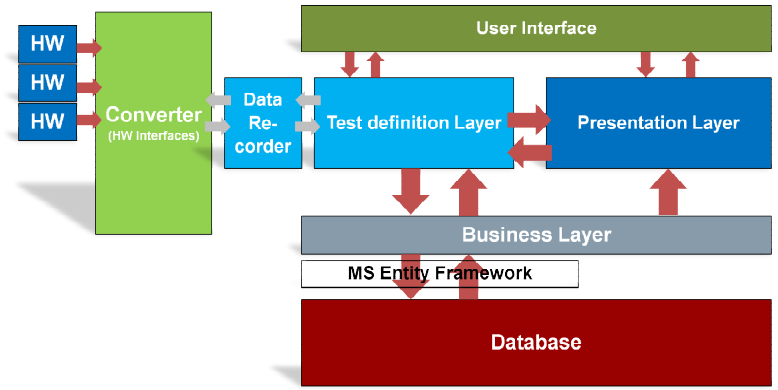
\includegraphics[width=0.7\textwidth]{SystemviewFTC}
	\caption{Systemview des Fire Test Commander}
	\label{fig:SystemViewFTC}
\end{figure}

\subsection{Bestehende Datenbank}
Die Bestehende Datenbank des FTC ist sehr komplex und beinhaltet sogar eine Rechteverteilung. Da die neue Software um einiges Schlanker wird und auch nicht eine solch komplexe Struktur der Datenbank verlangt, werden nur teile der Bestehenden Datenbank entnommen, welche mit der Hardwareabstraktion zu tun hat. Dies gewährleisted, dass die Komponente, welche übernommen wird ohne Probleme weiterhin funktioniert. 
\subsection{Software Architektur}
Dies System grobstruktur ist von der bestehenden FTC Applikation übernommen worden und Sieht wie folgt aus (siehe Figure \ref{fig:SystemViewUDA}). Es soll im Vergleich zur FTC Applikation jedoch keine Hardware abstraktion mehr implementiert werden, da diese Schon vollkommen übernommen werden kann.
\begin{figure}[htbp] 
	\centering
	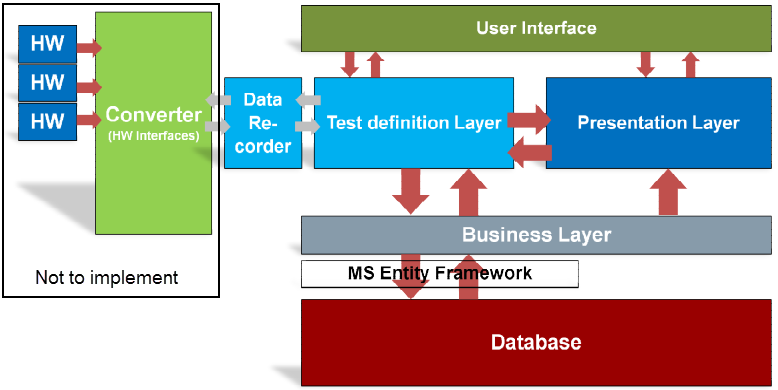
\includegraphics[width=0.7\textwidth]{Systemview}
	\caption{Systemview der UDA}
	\label{fig:SystemViewUDA}
\end{figure}
\subsubsection{Recorder}
\subsubsection{GUI / Tasks}
\subsubsection{Objek}
\subsection{Datenbank}
\subsubsection{Datenbank-Classen}
\subsection{Testing}
\section{Projektergebnisse}
\section{Arbeitsjournal}
\section{Fazit}
\section{Bestätigung Arbeitgeber}

\end{document}